\documentclass[a4paper, 11pt]{article}
\usepackage[utf8]{inputenc}
\usepackage[left=1in,right=1in,bottom=0.8in]{geometry}
\usepackage{enumitem}
\usepackage{graphicx}
\graphicspath{ {Figures/} }
\usepackage{float}
\usepackage[labelfont=bf]{caption}
\usepackage{fixltx2e}
\usepackage{caption}
\usepackage{amsmath}
\usepackage{capt-of}
\usepackage{minted}
\usepackage{tabu}
\let\svthefootnote\thefootnote

\title{\bf Experiment 5\\\vspace*{2mm} 8-Bit ALU on the Krypton CPLD}
\author{\it Dhruv Ilesh Shah | 150070016}
\date{February 17, 2017}

\begin{document}
\maketitle
\section*{Overview}
The ALU, or Arithmetic Logic Unit, is a very crucial part of any processor. By definition, it must be able to perform simple arithmetic and logical operations. In this experiment, I have implemented an 8-bit ALU which can perform the following operations.
\begin{enumerate}

	\item Addition
	\item Subtraction
	\item Left-Shift
	\item Right-Shift
\end{enumerate}

The code was compiled on Quartus Prime, and simulated using ModelSim. GHDL was also used for simulation purposes, at a low level. This was then uploaded to the {\em Krypton v1.1} 5M1270ZT144C5N CPLD-based board.

The codes and setup have been covered in section 1. We build the ALU piece-wise, by implementing each module independently. The VHDL codes have been kept modular and as generic as possible, for reusability and code clarity. Section 2 presents the simulation observations and miscellaneous results. Section 3 presents the observations after running the scan-chain test on the board.

\section{Setup}

The aim is to build an ALU with 4 different purposes. At a basic level, we can build 4 different modules and then use a 4-bit multiplexer to choose the final output of the ALU.
\begin{center}

\begin{tabular}{| c | c | c |}
\hline
\bf op\_code & \bf Operation & \bf Result  \\
\hline 
00 & Addition & $Z = X + Y$ \\
01 & Subtraction & $Z = X - Y$ \\
10 & Logical Right Shift & $Z = X >> Y$ \\
11 & Logical Left Shift & $Z = X << Y$ \\
\hline
\end{tabular}
\end{center}
Sticking to the design guidelines, the logic has been implemented using \emph{only} two-input AND, OR and NOT gates. In this section, I build the elements piece-wise in the earlier parts, and put them all together in the end to form the entity \texttt{alu}.

Before entering specific implementation, we see that the \emph{XOR} operation can be useful in logic, and hence I made an entity \texttt{myXOR} which can be used later on.
\inputminted{vhdl}{ALU_exp/xor.vhd}

This entity will be used multiple times in the various implementation below.
\subsection{Addition}

The addition operation can be carried out in multiple ways, but given the scale of the problem, and the possibility of scaling, reusability of the code is essential. I have implemented the 8-bit adder using 8 units of 1-bit \emph{full adders}. This can be extended using 2-bit full adders etc, to reduce the delays, but the complexity of implementation remains $\mathcal{O}(n)$. For a problem this size, the logarithmic adder would become too complex in space, and hence I stuck to the simpler model.

\subsubsection*{Full Adder}
Consider a block with inputs $c_i, x_i, y_i$ and outputs $c_o, s_o$.
\begin{equation}
\begin{split}
s_o &= c_i \oplus x_i \oplus y_i \\
c_o &= x_iy_i + y_ic_i + c_ix_i
\end{split}
\end{equation}
The implementation is given below as the entity \texttt{full\_adder}.

\inputminted[linenos]{vhdl}{ALU_exp/full_adder.vhd}


\subsubsection*{Eight Bit Adder}
Using this module, we can easily define the 8-bit addition operation as below. {\em (Note that I have avoided using loops as a structure, to keep the code raw, and close to how it is actually implemented in hardware. The redundancy can be easily be replaced by calling a process and iterating.)}

\inputminted[linenos]{vhdl}{ALU_exp/EightBitAdder.vhd}
\newpage
\subsection{Subtractor}
Approaching the subtractor in a manner similar to the adder, I have used a 1-bit full subtractor, which is then used to create an 8-bit subtractor.

\subsubsection*{Full Subtractor}
Consider a block with inputs $d_i, x_i, y_i$ and outputs $d_o, s_o$.
\begin{equation}
\begin{split}
s_o &= c_i \oplus x_i \oplus y_i \\
c_o &= \overline{x_i}y_i + d_i(\overline{x_i \oplus y_i})
\end{split}
\end{equation}
The implementation of the above is given below.
\inputminted[linenos]{vhdl}{ALU_exp/subtractor.vhd}
\subsubsection*{Eight Bit Subtractor}
By using the above unit entity, and extending the definition of the subtractor to 8 bits, we have the following.
\inputminted[linenos]{vhdl}{ALU_exp/EightBitSubtractor.vhd}


\subsection{Logical Right Shift}
The logical right shift is an essential operation for an ALU. One of the simplest interpretation can be division by 2. This can give an easy way to implement multiplication/division operations. Hardwiring is always an option, but a more general and reusable algorithm would be preferred.

For this purpose, I perform shifts using \emph{logarithmic barrel shifting}. An illustration of barrel-shifting is given in figure 1. Note that although both $X, Y$ are 8-bit, if $Y$ is more than $111$, then the output would be monotonously zero (not a rotator). Hence we need to implement only 3 stages.

\begin{figure}[h]
\centering
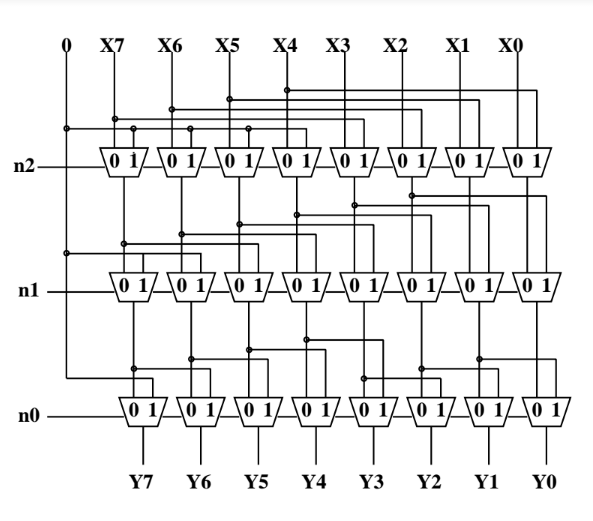
\includegraphics[scale=0.6]{barrel_right}
\caption{Logical Right Shift (\emph{Barrel Shift})}
\end{figure}
We notice that an important feature of this implementation is the multiplexer. So, I begin by creating a \texttt{mux} entity, which is then used to make the 8-mux chains, eventually making our shifter.

\subsubsection*{MUX}
A multiplexer with inputs $n_1,n_0,s$ and output $b$ follows:
$$
b = s n_1 + \overline{s}n_0
$$
\inputminted[linenos]{vhdl}{ALU_exp/mux.vhd}

\subsubsection*{MUX Chains}
In principle, we can use a generic 8-unit chain of multiplexers with 16 inputs and 8 outputs, working the way we like. Such an implementation is given below.

\inputminted[linenos]{vhdl}{ALU_exp/mux8.vhd}

In this implementation, we would have to give the input vector in the order they enter, and hence the code would end up messy anyway. Instead, I made three different entities \texttt{mux\_chain\_1  mux\_chain\_2  mux\_chain\_3} customised to the chains seen in the diagram.\\


\textbf{MUX Chain 1 ($n_2$)}\\
\inputminted[linenos]{vhdl}{ALU_exp/mux_chain_1.vhd}
\newpage
\textbf{MUX Chain 2 ($n_1$)}\\
\inputminted[linenos]{vhdl}{ALU_exp/mux_chain_2.vhd}

\textbf{MUX Chain 3 ($n_0$)}\\
\inputminted[linenos]{vhdl}{ALU_exp/mux_chain_3.vhd}

\subsubsection*{Right Barrel Shifter}
Now that we have these components ready, we can code up the shifter.

\inputminted[linenos]{vhdl}{ALU_exp/right_shifter.vhd}

\subsection{Logical Left Shifter}
Instead of designing the left shifter from scratch, we can use symmetry arguments to ease our process. Given a right shifter, feeding it with the reverse of the input vector, and reading the reverse of its output vector gives the same result as an intended left shifter! This means that all we need is a way to reverse the vector. The rest is straightforward.\\

Instead of writing the reverse operations within the main body, I have used another entity \texttt{reverse} for clarity.
\subsubsection*{8-bit Reverse}
 
 The logic is straightforward, as given below.
 \inputminted[linenos]{vhdl}{ALU_exp/8bit_rev.vhd}

\subsubsection*{Left Barrel Shifter}
Given the \texttt{right\_shifter} from above, and the \texttt{reverse} entity, we can perform this very easily.
\inputminted[linenos]{vhdl}{ALU_exp/left_shifter.vhd}
\subsection{The ALU}
Putting together the whole code, we declare the \texttt{alu} entity as follows.\\
{\em(Most of this segment was provided by WEL and hence the use of \texttt{if...else}. This can easily be replaced by multiplexers.)}

\inputminted[linenos]{vhdl}{ALU_exp/my_alu.vhd}
The \textbf{Testbench} used for this entire setup is also given below.
\inputminted[linenos]{vhdl}{ALU_exp/Testbench.vhd}

\newpage
\section{Observations}
In this section, we simulate the above codes to test logic and observe the delay characteristics.
\subsection{Addition}
Figures 2-3 show the results of the simulation. \emph{(Since the number of possible test cases is too large ($2^{16}$), I have showed a small section of the waveform.)}

\begin{figure}[h]
\centering
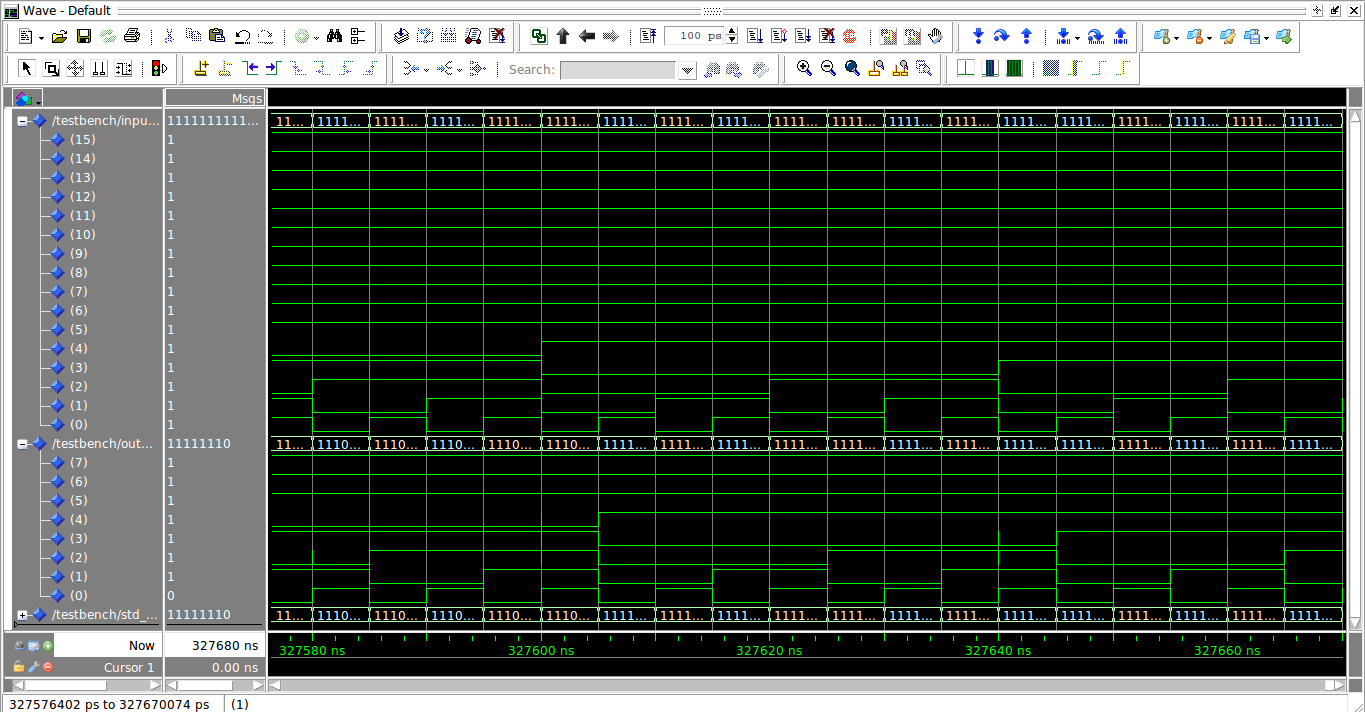
\includegraphics[scale=0.33]{Adder_RTL}
\caption{RTL Simulation of the Addition operation}
\end{figure}

\begin{figure}[H]
\centering
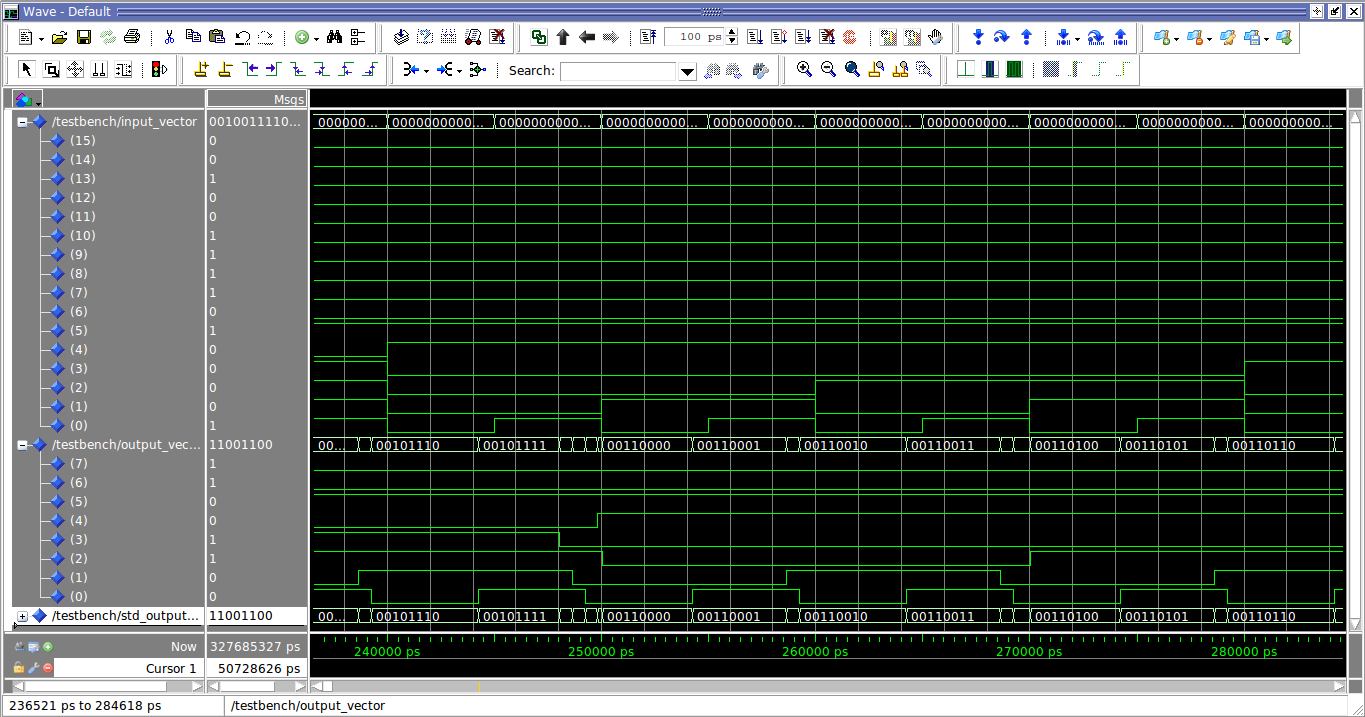
\includegraphics[scale=0.33]{Adder_Gate}
\caption{Gate-level Simulation of the Addition operation}
\end{figure}

\newpage
\subsection{Subtraction}
Figures 4-5 show the results of the simulation. \emph{(Since the number of possible test cases is too large ($2^{16}$), I have showed a small section of the waveform.)}

\begin{figure}[H]
\centering
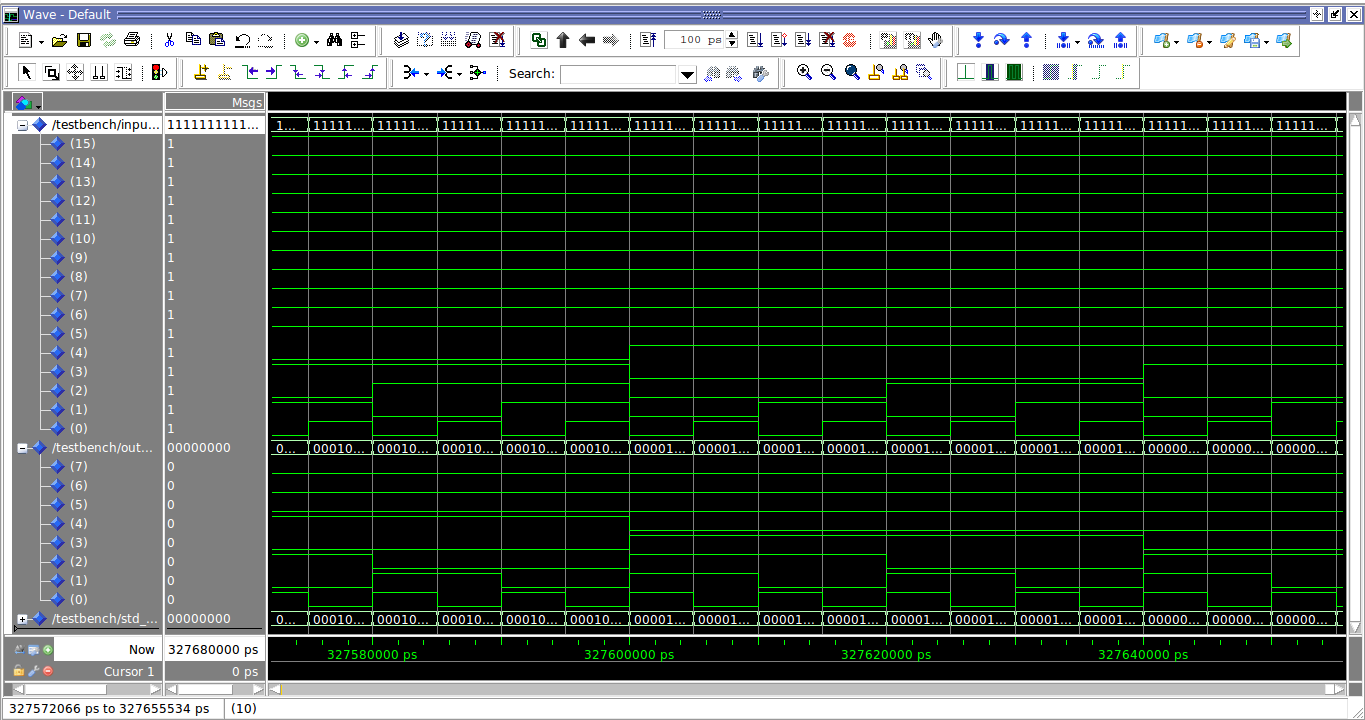
\includegraphics[scale=0.33]{Subtractor_RTL}
\caption{RTL Simulation of the Subtraction operation}
\end{figure}

\begin{figure}[H]
\centering
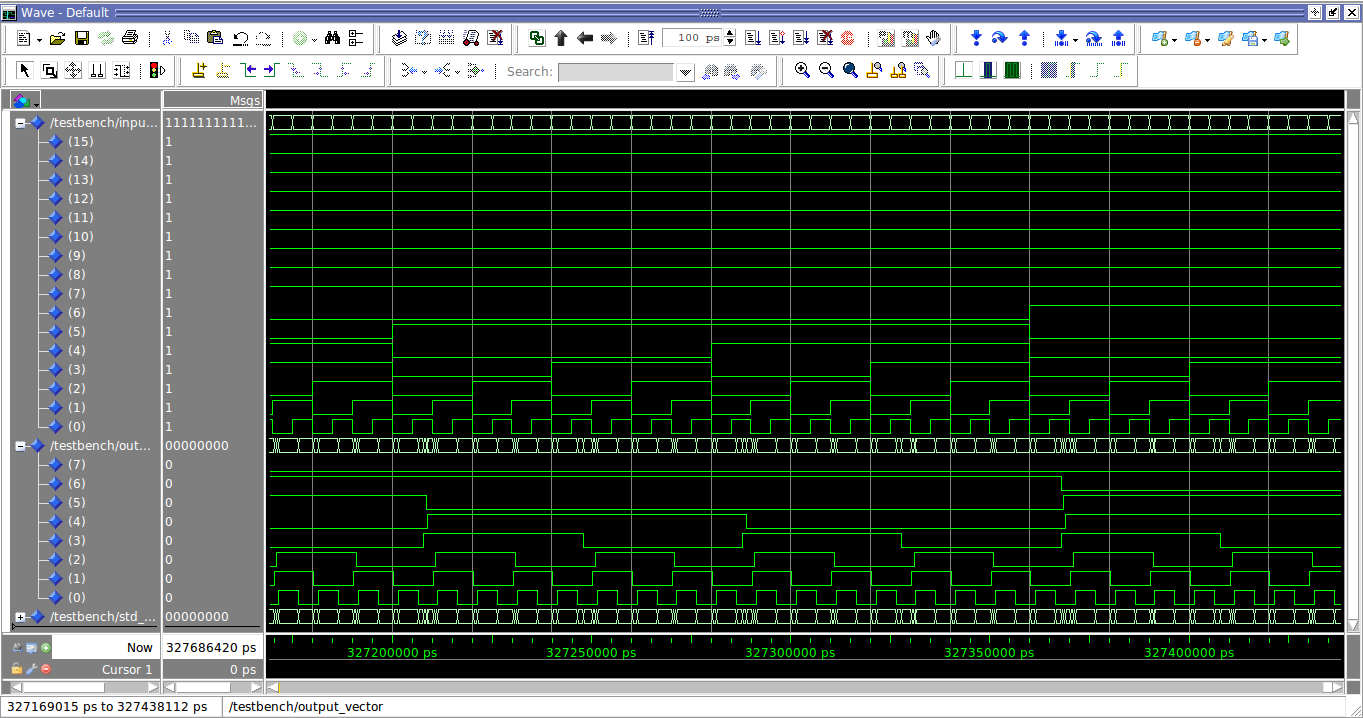
\includegraphics[scale=0.33]{Subtractor_Gate}
\caption{Gate-level Simulation of the Subtraction operation}
\end{figure}

\newpage
\subsection{Logical Right Shift}
Figures 6-7 show the results of the simulation. \emph{(Since the number of possible test cases is too large ($2^{16}$), I have showed a small section of the waveform.)}

\begin{figure}[H]
\centering
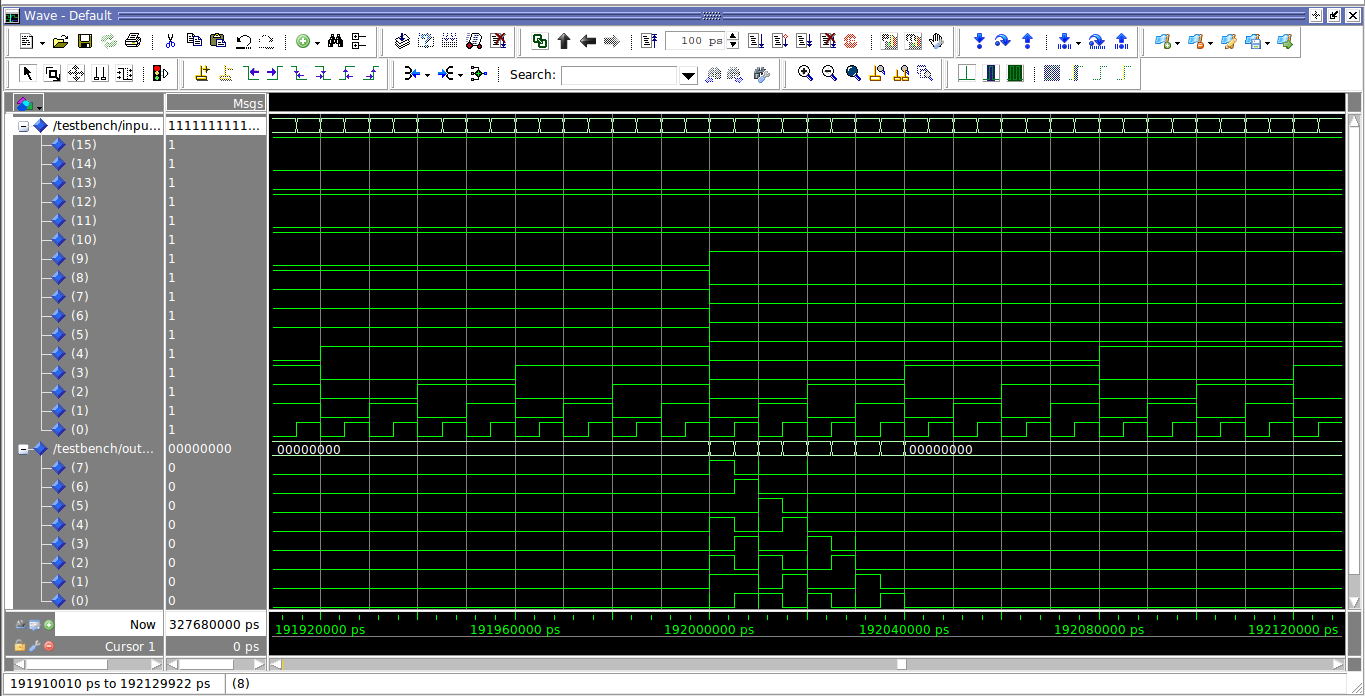
\includegraphics[scale=0.33]{rightshift_RTL}
\caption{RTL Simulation of the Logical Right Shift operation}
\end{figure}

\begin{figure}[H]
\centering
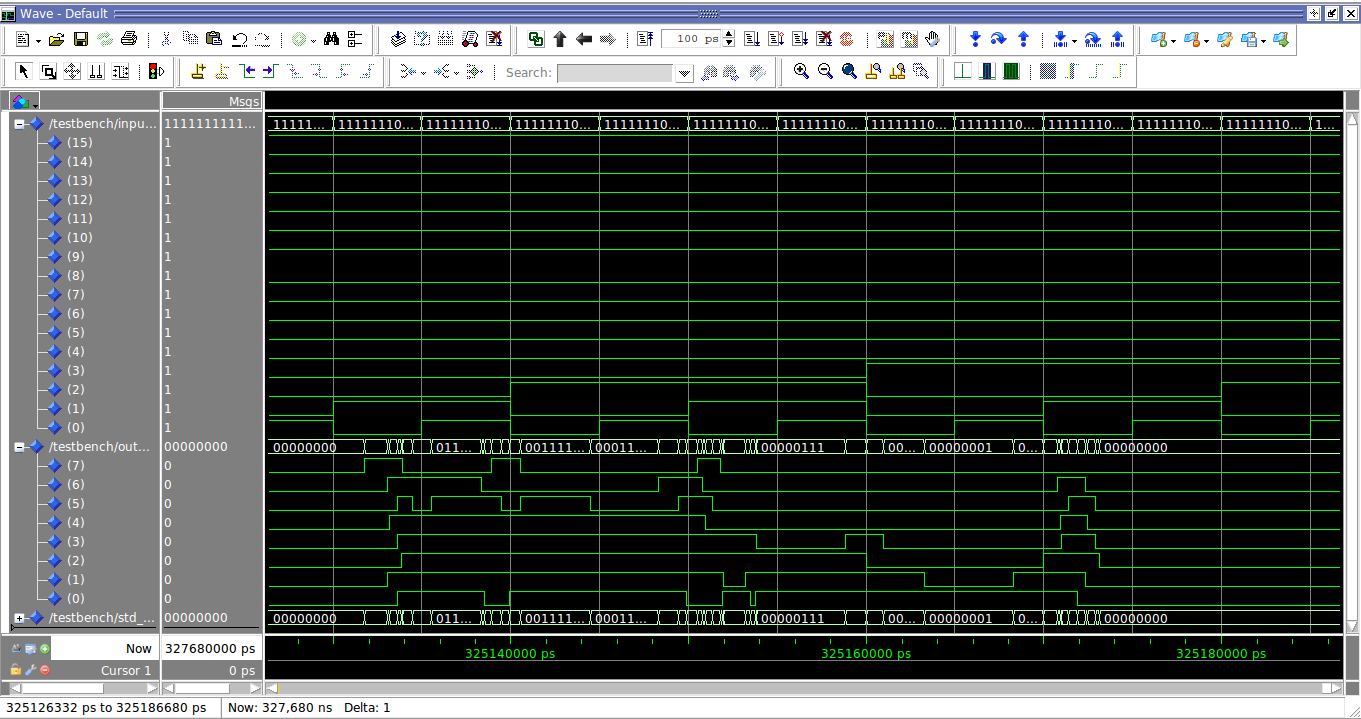
\includegraphics[scale=0.33]{rightshift_Gate}
\caption{Gate-level Simulation of the Logical Right Shift operation}
\end{figure}

\newpage
\subsection{Logical Left Shift}
Figures 8-9 show the results of the simulation. \emph{(Since the number of possible test cases is too large ($2^{16}$), I have showed a small section of the waveform.)}

\begin{figure}[H]
\centering
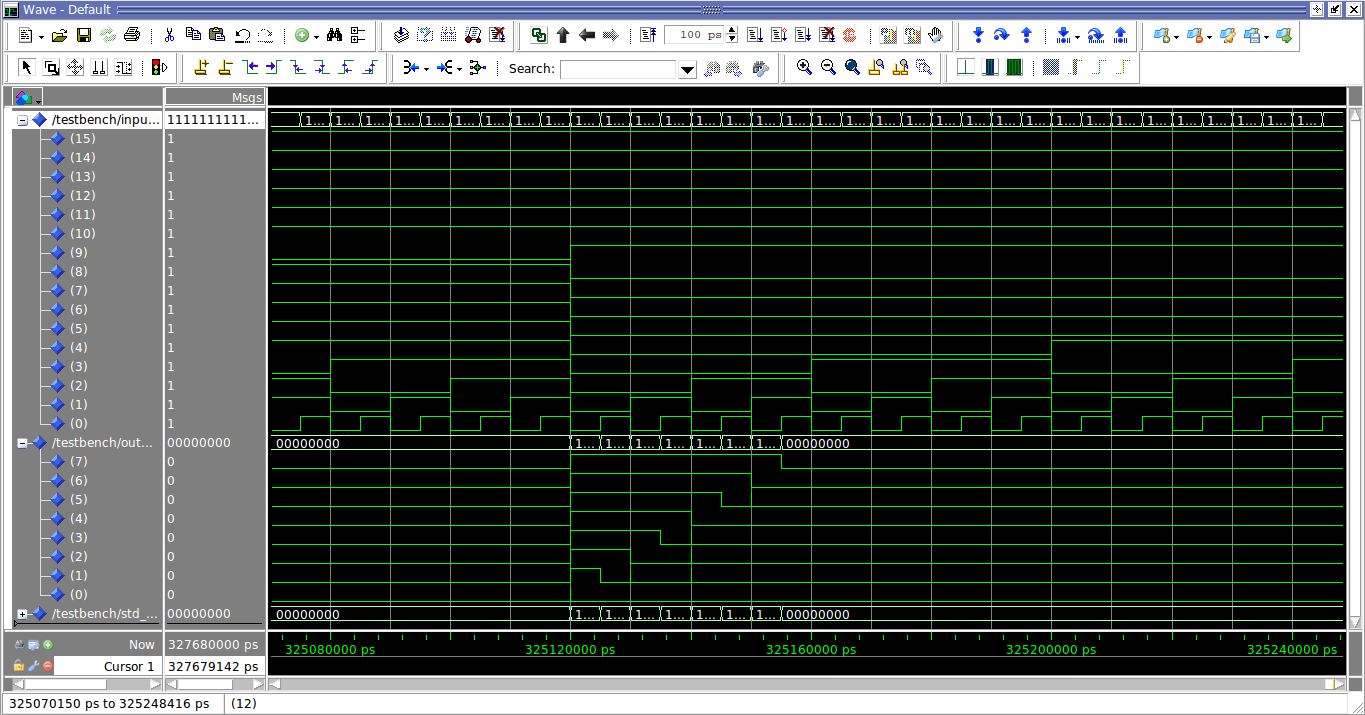
\includegraphics[scale=0.33]{leftshift_RTL}
\caption{RTL Simulation of the Logical Left Shift operation}
\end{figure}

\begin{figure}[H]
\centering
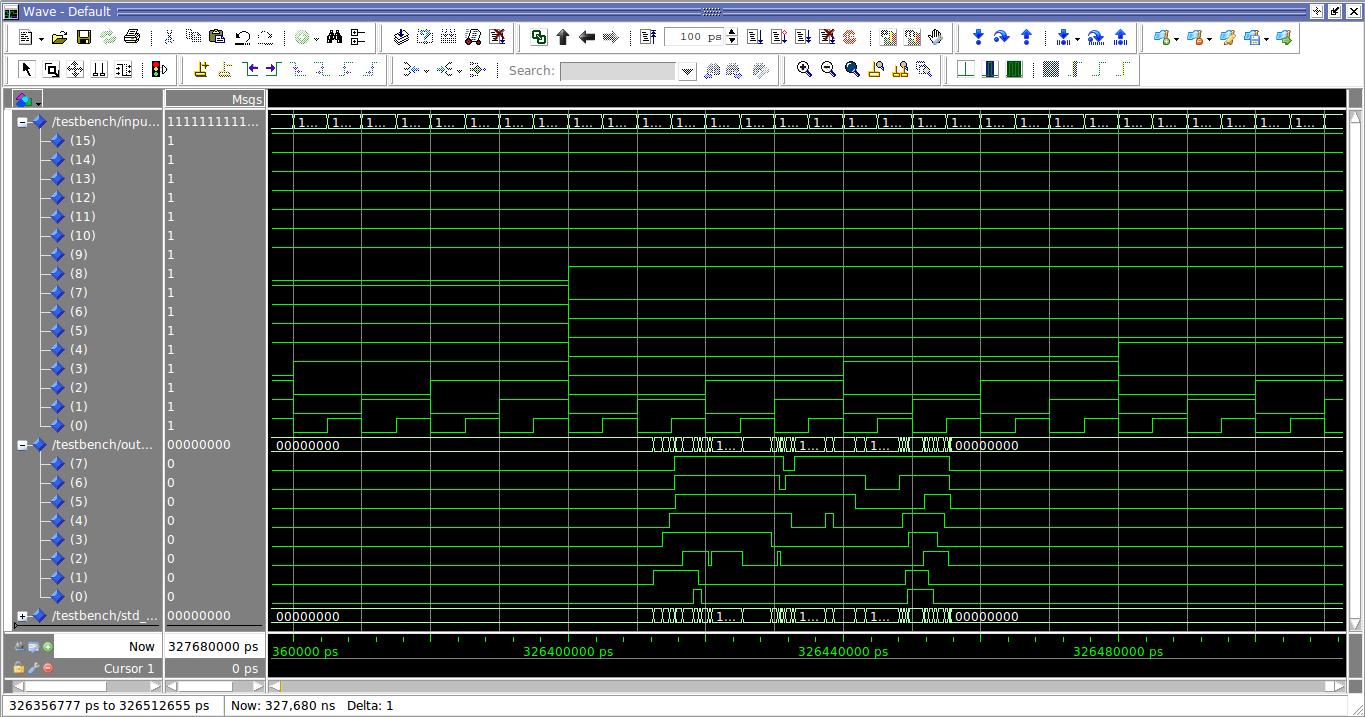
\includegraphics[scale=0.33]{leftshift_Gate}
\caption{Gate-level Simulation of the Logical Left Shift operation}
\end{figure}

\newpage
\section{Scan-Chain Tests}

We have tested the logic using the RTL simulations, emulated the CPLD performance using the gate-level simulation and uploaded the code on the Krypton board. Next, we need to check that the code is actually running as it is expected to, on the board. We could do so manually but that is not feasible due to the following reasons.
\begin{itemize}
	\item Our current circuit requires 18 control switches. In any given setup, it \emph{may} not be possible to allocate as many I/O pins. As the complexity increases, it will indeed not be possible to allocate so many pins.
	\item Even if the above is possible, the total number of test cases is \emph{exponential} in the size of the input and it is impractical to perform each of this manually.\footnote{It is not wise to skip any case because, say, we do miss out a failed case it can cascade into unimaginable consequences, which can become difficult to debug.}
\end{itemize}

Hence, we test the uploaded code on the hardware using the scan-chain setup, as suggested in the manual. This setup was run first on a small sample of test cases to check common logic errors. Later on, exhaustive tests ($2^{18}$) were performed to check for any issues on the overall performance.

\subsection*{Results}
\subsubsection*{Sample Tests}
\begin{figure}[H]
\centering
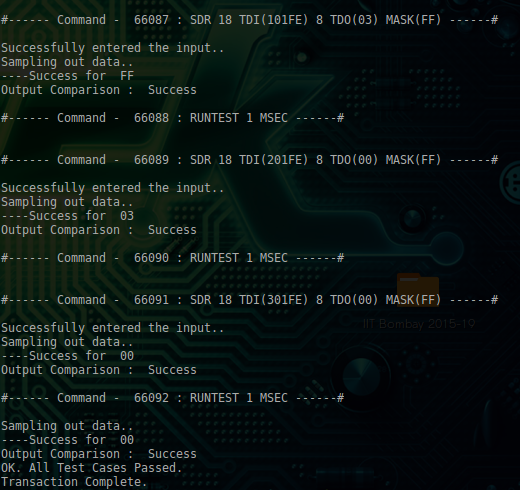
\includegraphics[scale=0.66]{Complete_Test}
\caption{Results of the scan-chain test for random sample test cases.}
\end{figure}

\subsubsection*{Exhaustive Tests}
\begin{figure}[H]
\centering
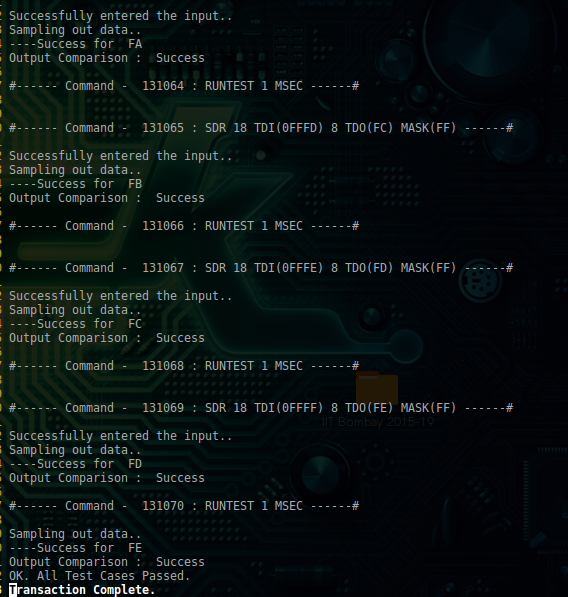
\includegraphics[scale=0.66]{Add_Exhaustive}
\caption{Results of the scan-chain test on an exhaustive set of inputs.}
\end{figure}

\section*{Conclusion}
Starting from the very scratch, in this report, I have presented the logic and code for an 8-bit ALU as required. The logic was tested using RTL simulation, followed by the gate-level simulation for delay analysis and emulating the CPLD. This was followed by an actual rigorous test on the CPLD board after burning the code on it, using the \emph{TIVA-C} microcontroller.
\par
All the cases passed successfully at all stages and hence the complete ALU can be used in hardware, as required.

\end{document}
